\pagebreak

A prototipagem foi realizada com o objetivo de criar uma interface amigável e funcional para os usuários do sistema. Foram desenvolvidas telas para diferentes funcionalidades, permitindo uma interação intuitiva e eficiente.

\subsection{Consultas}

As telas de consulta foram desenvolvidas para permitir que o usuário visualize e gerencie suas consultas médicas:

\begin{figure}[!htbp]
	\centering
	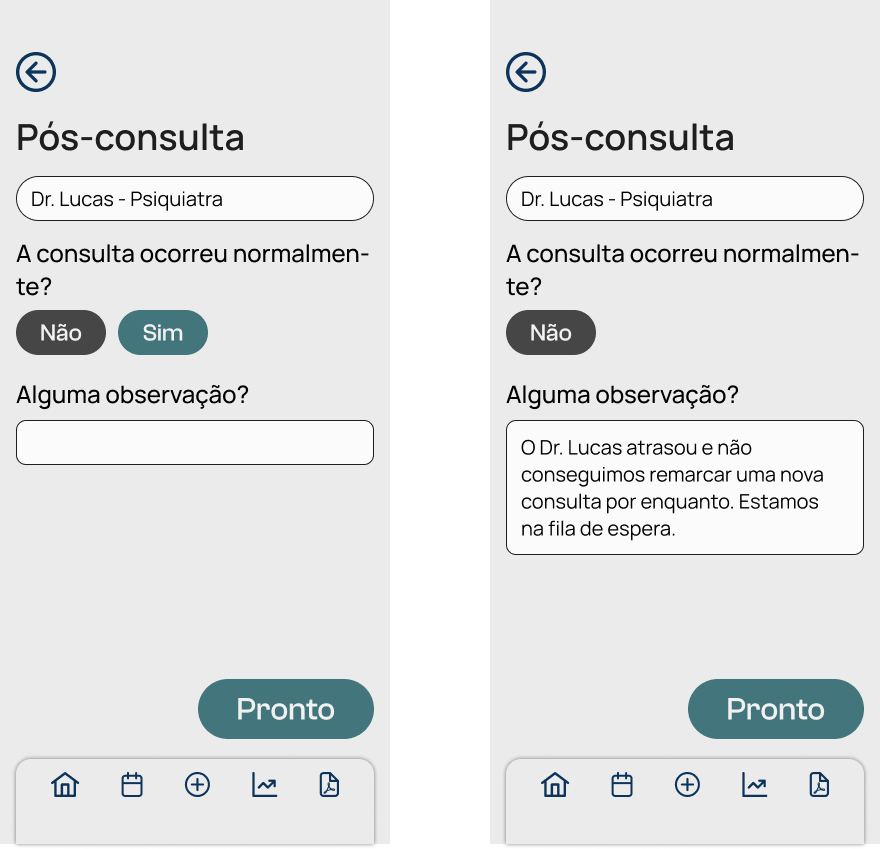
\includegraphics[width=1.0\linewidth]{MyMed - Modelagem/Avaliação Consulta.png}
	\caption{Avaliação de Consulta}
	\fonte{Autores.}
	\label{avaliacao_consulta}
\end{figure}

\subsection{Calendário}

As telas de calendário foram projetadas para ajudar o usuário a visualizar e gerenciar suas consultas médicas de forma eficiente:

\begin{figure}[!htbp]
	\centering
	\includegraphics[width=0.6\linewidth]{MyMed - Modelagem/Calendário - Consulta Finalizada-1.png}
	\caption{Calendário - Consulta Finalizada 1}
	\fonte{Autores.}
	\label{calendario_consulta_finalizada_1}
\end{figure}

\begin{figure}[!htbp]
	\centering
	\includegraphics[width=0.6\linewidth]{MyMed - Modelagem/Calendário - Consulta Finalizada.png}
	\caption{Calendário - Consulta Finalizada}
	\fonte{Autores.}
	\label{calendario_consulta_finalizada}
\end{figure}

\begin{figure}[!htbp]
	\centering
	\includegraphics[width=0.6\linewidth]{MyMed - Modelagem/Calendário.png}
	\caption{Calendário}
	\fonte{Autores.}
	\label{calendario}
\end{figure}

\subsection{Gráficos}

As telas de gráficos foram desenvolvidas para fornecer uma visualização clara e intuitiva dos dados de saúde do usuário:

\begin{figure}[!htbp]
	\centering
	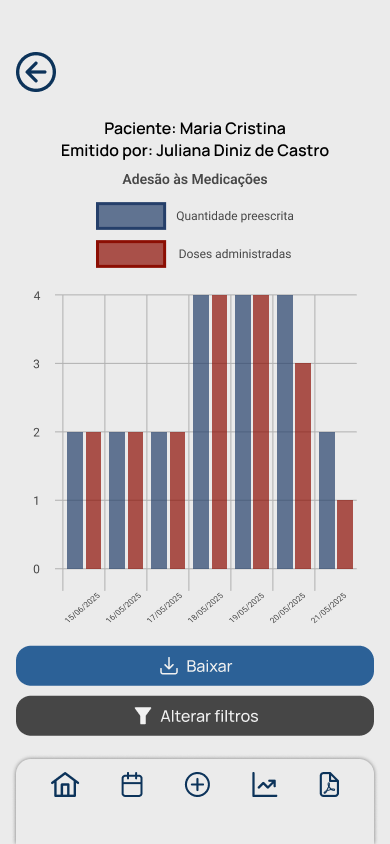
\includegraphics[width=0.6\linewidth]{MyMed - Modelagem/Gráfico - Adesão a Medicações.png}
	\caption{Gráfico - Adesão a Medicações}
	\fonte{Autores.}
	\label{grafico_adesao_medicacoes}
\end{figure}

\begin{figure}[!htbp]
	\centering
	\includegraphics[width=0.6\linewidth]{MyMed - Modelagem/Gráfico - Glicemia.png}
	\caption{Gráfico - Glicemia}
	\fonte{Autores.}
	\label{grafico_glicemia}
\end{figure}

\begin{figure}[!htbp]
	\centering
	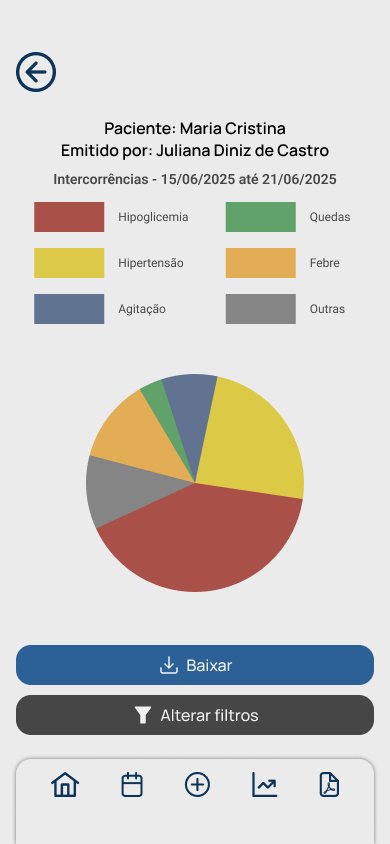
\includegraphics[width=0.6\linewidth]{MyMed - Modelagem/Gráfico - Intercorrências.png}
	\caption{Gráfico - Intercorrências}
	\fonte{Autores.}
	\label{grafico_intercorrencias}
\end{figure}

\begin{figure}[!htbp]
	\centering
	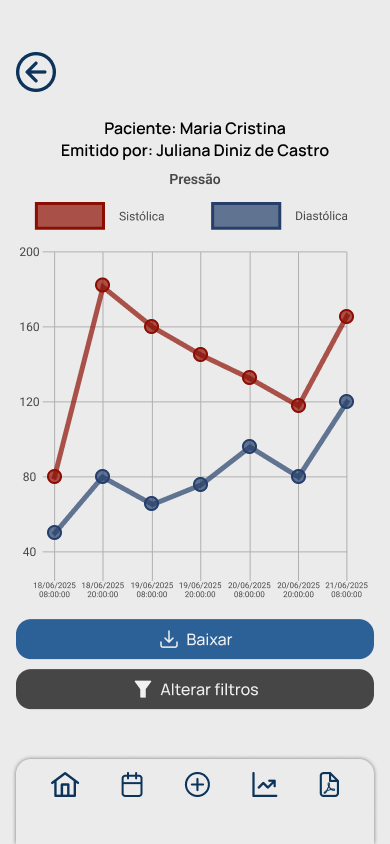
\includegraphics[width=0.6\linewidth]{MyMed - Modelagem/Gráfico - Pressão.png}
	\caption{Gráfico - Pressão}
	\fonte{Autores.}
	\label{grafico_pressao}
\end{figure}

\begin{figure}[!htbp]
	\centering
	\includegraphics[width=0.6\linewidth]{MyMed - Modelagem/Gráficos.png}
	\caption{Gráficos}
	\fonte{Autores.}
	\label{graficos}
\end{figure}

\subsection{Login e Perfil}

As telas de login e perfil foram projetadas para garantir uma experiência de usuário segura e personalizada:

\begin{figure}[!htbp]
	\centering
	
\includegraphics[width=0.6\linewidth]{MyMed - Modelagem/Login.png}
	\caption{Login}
	\fonte{Autores.}
	\label{login}
\end{figure}

\begin{figure}[!htbp]
	\centering
	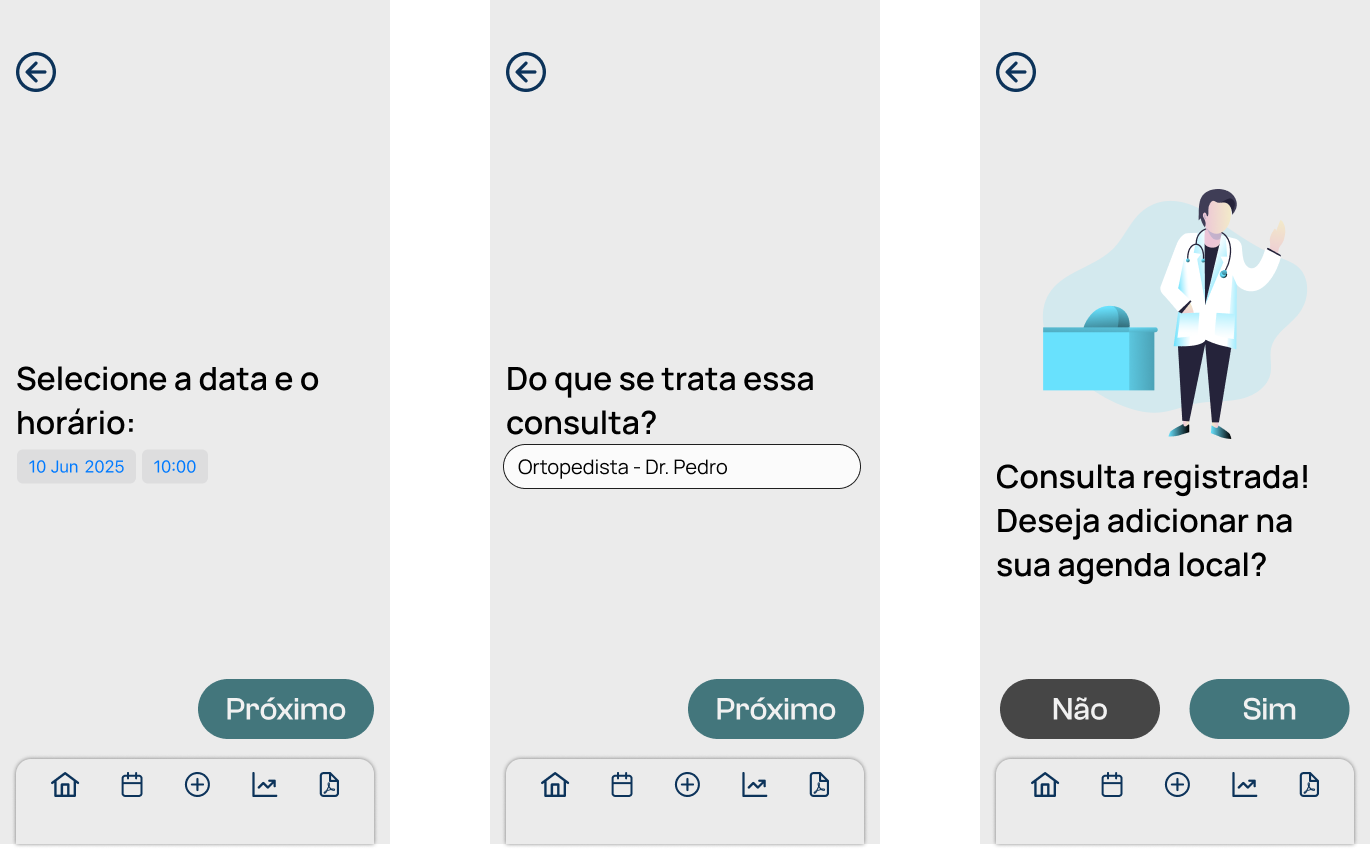
\includegraphics[width=1.0\linewidth]{MyMed - Modelagem/Nova Consulta.png}
	\caption{Nova Consulta}
	\fonte{Autores.}
	\label{nova_consulta}
\end{figure}

\begin{figure}[!htbp]
	\centering
	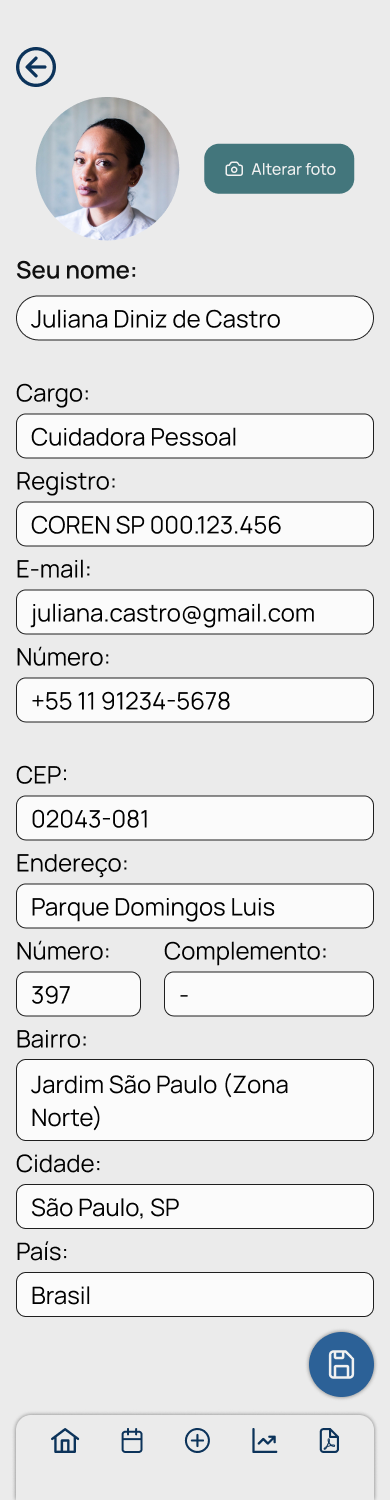
\includegraphics[width=0.35\linewidth]{MyMed - Modelagem/Perfil - Edição.png}
	\caption{Perfil - Edição}
	\fonte{Autores.}
	\label{perfil_edicao}
\end{figure}

\begin{figure}[!htbp]
	\centering
	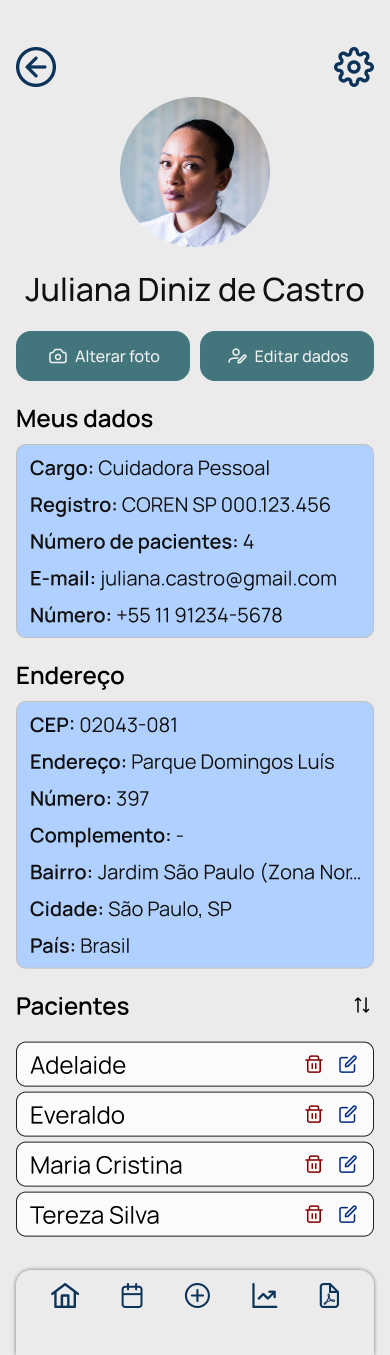
\includegraphics[width=0.35\linewidth]{MyMed - Modelagem/Perfil.png}
	\caption{Perfil}
	\fonte{Autores.}
	\label{perfil}
\end{figure}

\begin{figure}[!htbp]
	\centering
	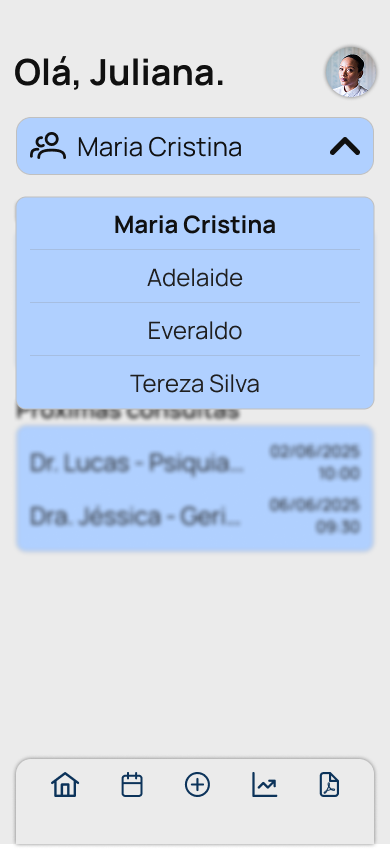
\includegraphics[width=0.6\linewidth]{MyMed - Modelagem/Tela Inicial - Dropdown Nomes.png}
	\caption{Tela Inicial - Dropdown Nomes}
	\fonte{Autores.}
	\label{tela_inicial_dropdown_nomes}
\end{figure}

\subsection{Tela Inicial}

A tela inicial do aplicativo \nomeprojeto foi projetada para ser intuitiva e fácil de navegar, permitindo que os usuários acessem rapidamente as funcionalidades principais:

\begin{figure}[!htbp]
	\centering
	\includegraphics[width=0.6\linewidth]{MyMed - Modelagem/Tela Inicial (Botão +).png}
	\caption{Tela Inicial (Botão +)}
	\fonte{Autores.}
	\label{tela_inicial_botao_mais}
\end{figure}

\begin{figure}[!htbp]
	\centering
	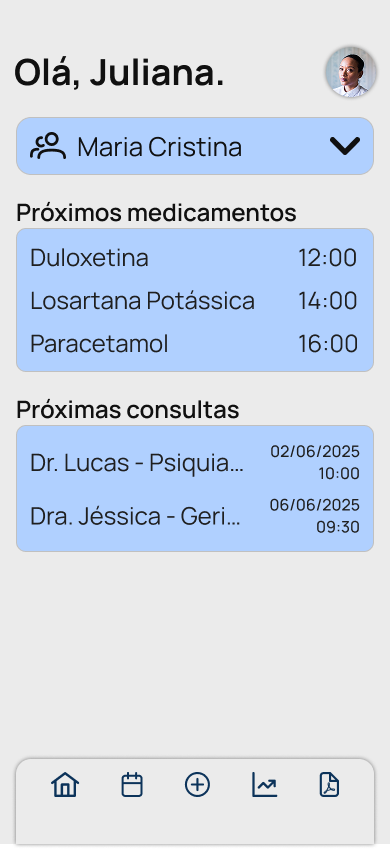
\includegraphics[width=0.6\linewidth]{MyMed - Modelagem/Tela Inicial.png}
	\caption{Tela Inicial}
	\fonte{Autores.}
	\label{tela_inicial}
\end{figure}
